\documentclass[xcolor=dvipsnames,12pt]{beamer}

%\usepackage{amsmath,amsthm,amssymb,graphicx}

\mode<presentation>
{
  \usetheme{Rochester}
  %\usecolortheme[named=DarkSlateGray]{structure}
  % or ...
  \definecolor{baruch blue}{RGB}{9,39,105}
  \setbeamercolor{palette primary}{bg=baruch blue,fg=White}
  \setbeamercolor{palette secondary}{fg=Green,bg=Orange}
  \setbeamercolor{palette tertiary}{fg=Yellow,bg=Red}
  %\setbeamercolor{palette quatenary}{fg=Yellow,bg=Red}
  \setbeamercolor{block title}{fg=Green,bg=Black}
  \setbeamercolor{block title example}{fg=Yellow}
  \setbeamercolor{normal text}{fg=baruch blue}
% \setbeamercovered{transparent}
  % or whatever (possibly just delete it)
  \setbeamercolor{frametitle right}{bg=baruch blue!50!White,fg=White}
  \setbeamercolor{author in head/foot}{bg=baruch blue!50!White,fg=White}
}

\usepackage{amsmath}
\usepackage{amssymb}
\usepackage{graphicx}
\usepackage{amsthm}
\usepackage{bbm}
\usepackage{bm}
\usepackage{subcaption}

% \usepackage{biblatex}
% \usepackage[style=apa,doi=false]{biblatex}
% \addbibresource{lit.bib}
%\graphicspath{{../../../../../Google\ Drive/Projects/LinkEquate/Analysis/}}

\newcommand{\mbf}[1]{\boldsymbol{#1}}
\newcommand{\rank}{\varrho}
\newcommand{\thresh}{\tau}
\newcommand{\one}{\mbf{1}}
\newcommand{\comment}[1]{}


\title{A probabilistic graphical model for joint modeling of item response and process}
\author{Xiang Liu}
\institute{Educational Testing Service}
\date{\today}
\logo{\includegraphics[height=.8cm]{ETS_logo.jpg}}

\begin{document}
  \titlepage
  
  \begin{frame}
    \tableofcontents
  \end{frame}
  
  \section{Background}
  \begin{frame}{Background}
    \begin{itemize}
      \item Various process data becomes increasingly available, thanks to the improved digital assessment platforms.
      \item NAEP digital assessments.
      \item In addition to the traditional item responses, how do we make sense of the process data in large scale?
    \end{itemize}
  \end{frame}

  \begin{frame}{Example: calculator use}
    \begin{itemize}
      \item On-screen calculator for math items.
      \item The behaviors captured in the process data may relate to both item response and proficiency.
      \item The additional information from process data could prove to be useful in improving measurement precision as well as leading to better understanding the cognitive process of students.
      \item Develop a modeling approach that could simultaneously consider item response and process data.
      \item 2017 NAEP math assessment release block - grade 8.
    \end{itemize}
  \end{frame}

  \section{Descriptives and motivation}
  \begin{frame}{Data summary}
    \begin{itemize}
      \item The block consists of 19 items.
      \item Over $30,000$ students.
      \item A random sample of $3,000$ students.
      \item Some items have few calculator use, i.e. less than 30.
      \item I used 15 items.
    \end{itemize}
  \end{frame}

  \begin{frame}{Figure: calculator use by item}
    \begin{figure}
      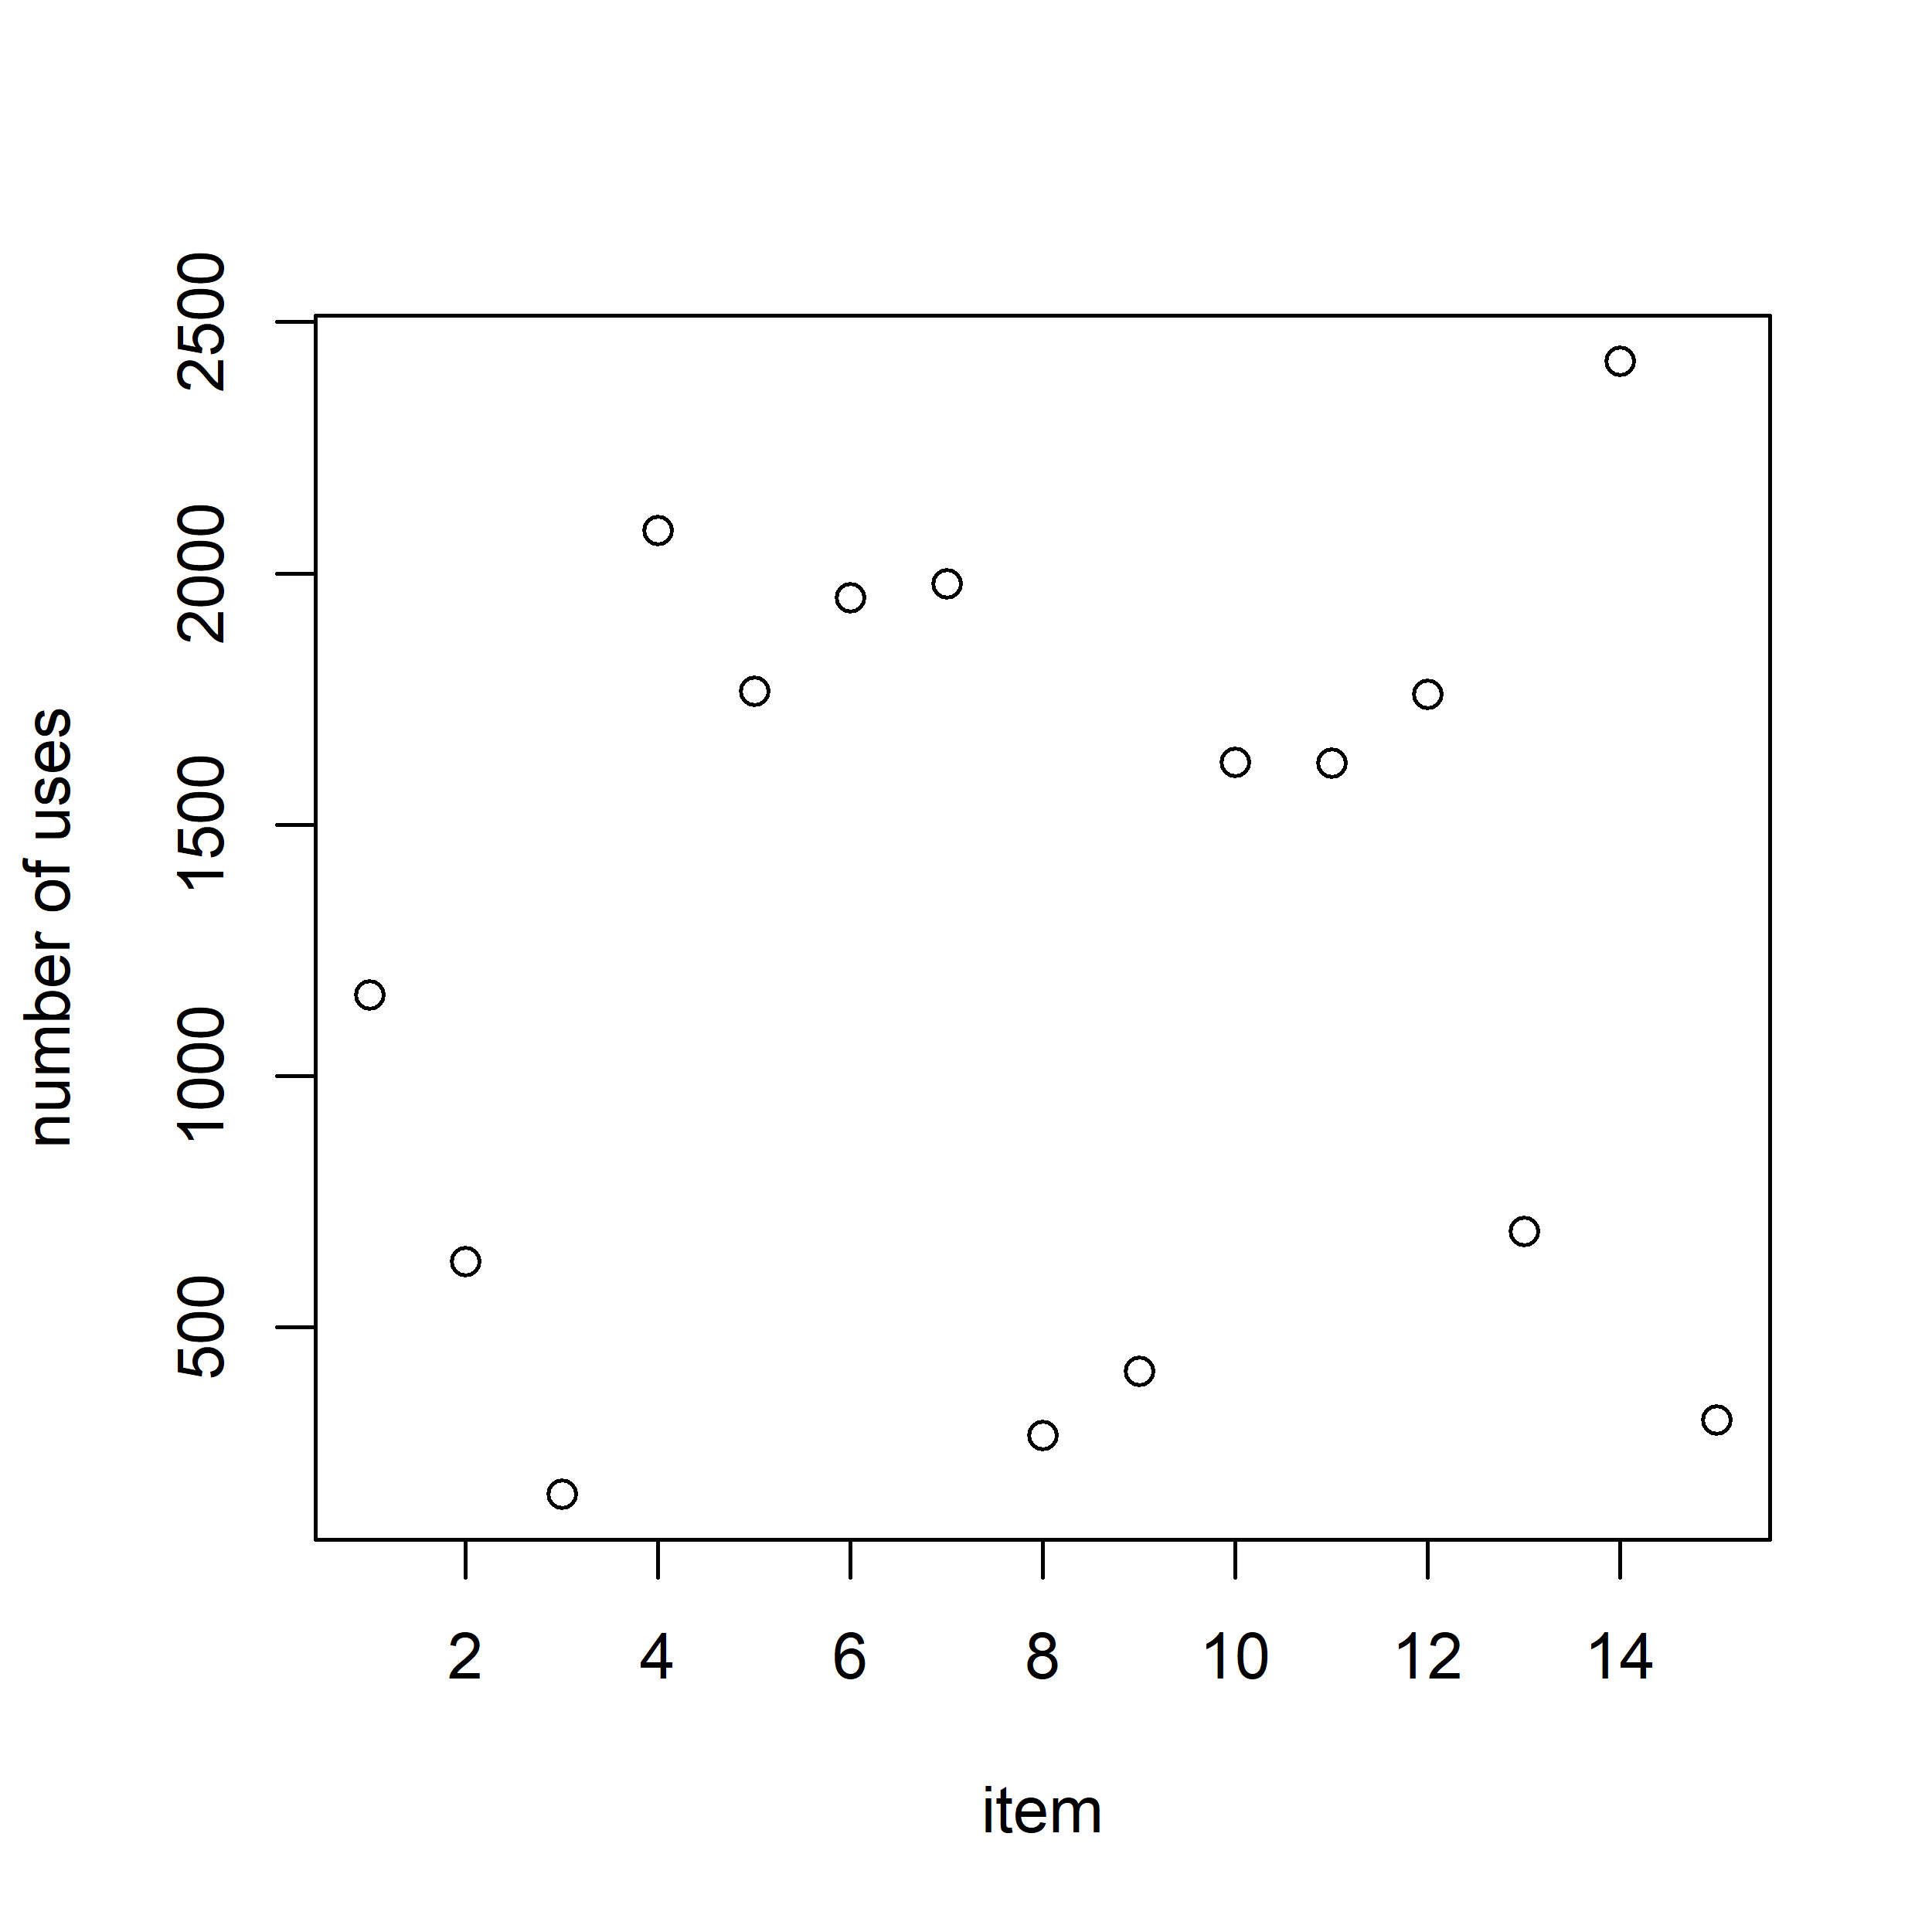
\includegraphics[scale = 0.5]{figures/cal_use_by_item.png}
    \end{figure}
  \end{frame}

  \begin{frame}{Figure: calculator use by student}
    \begin{figure}
      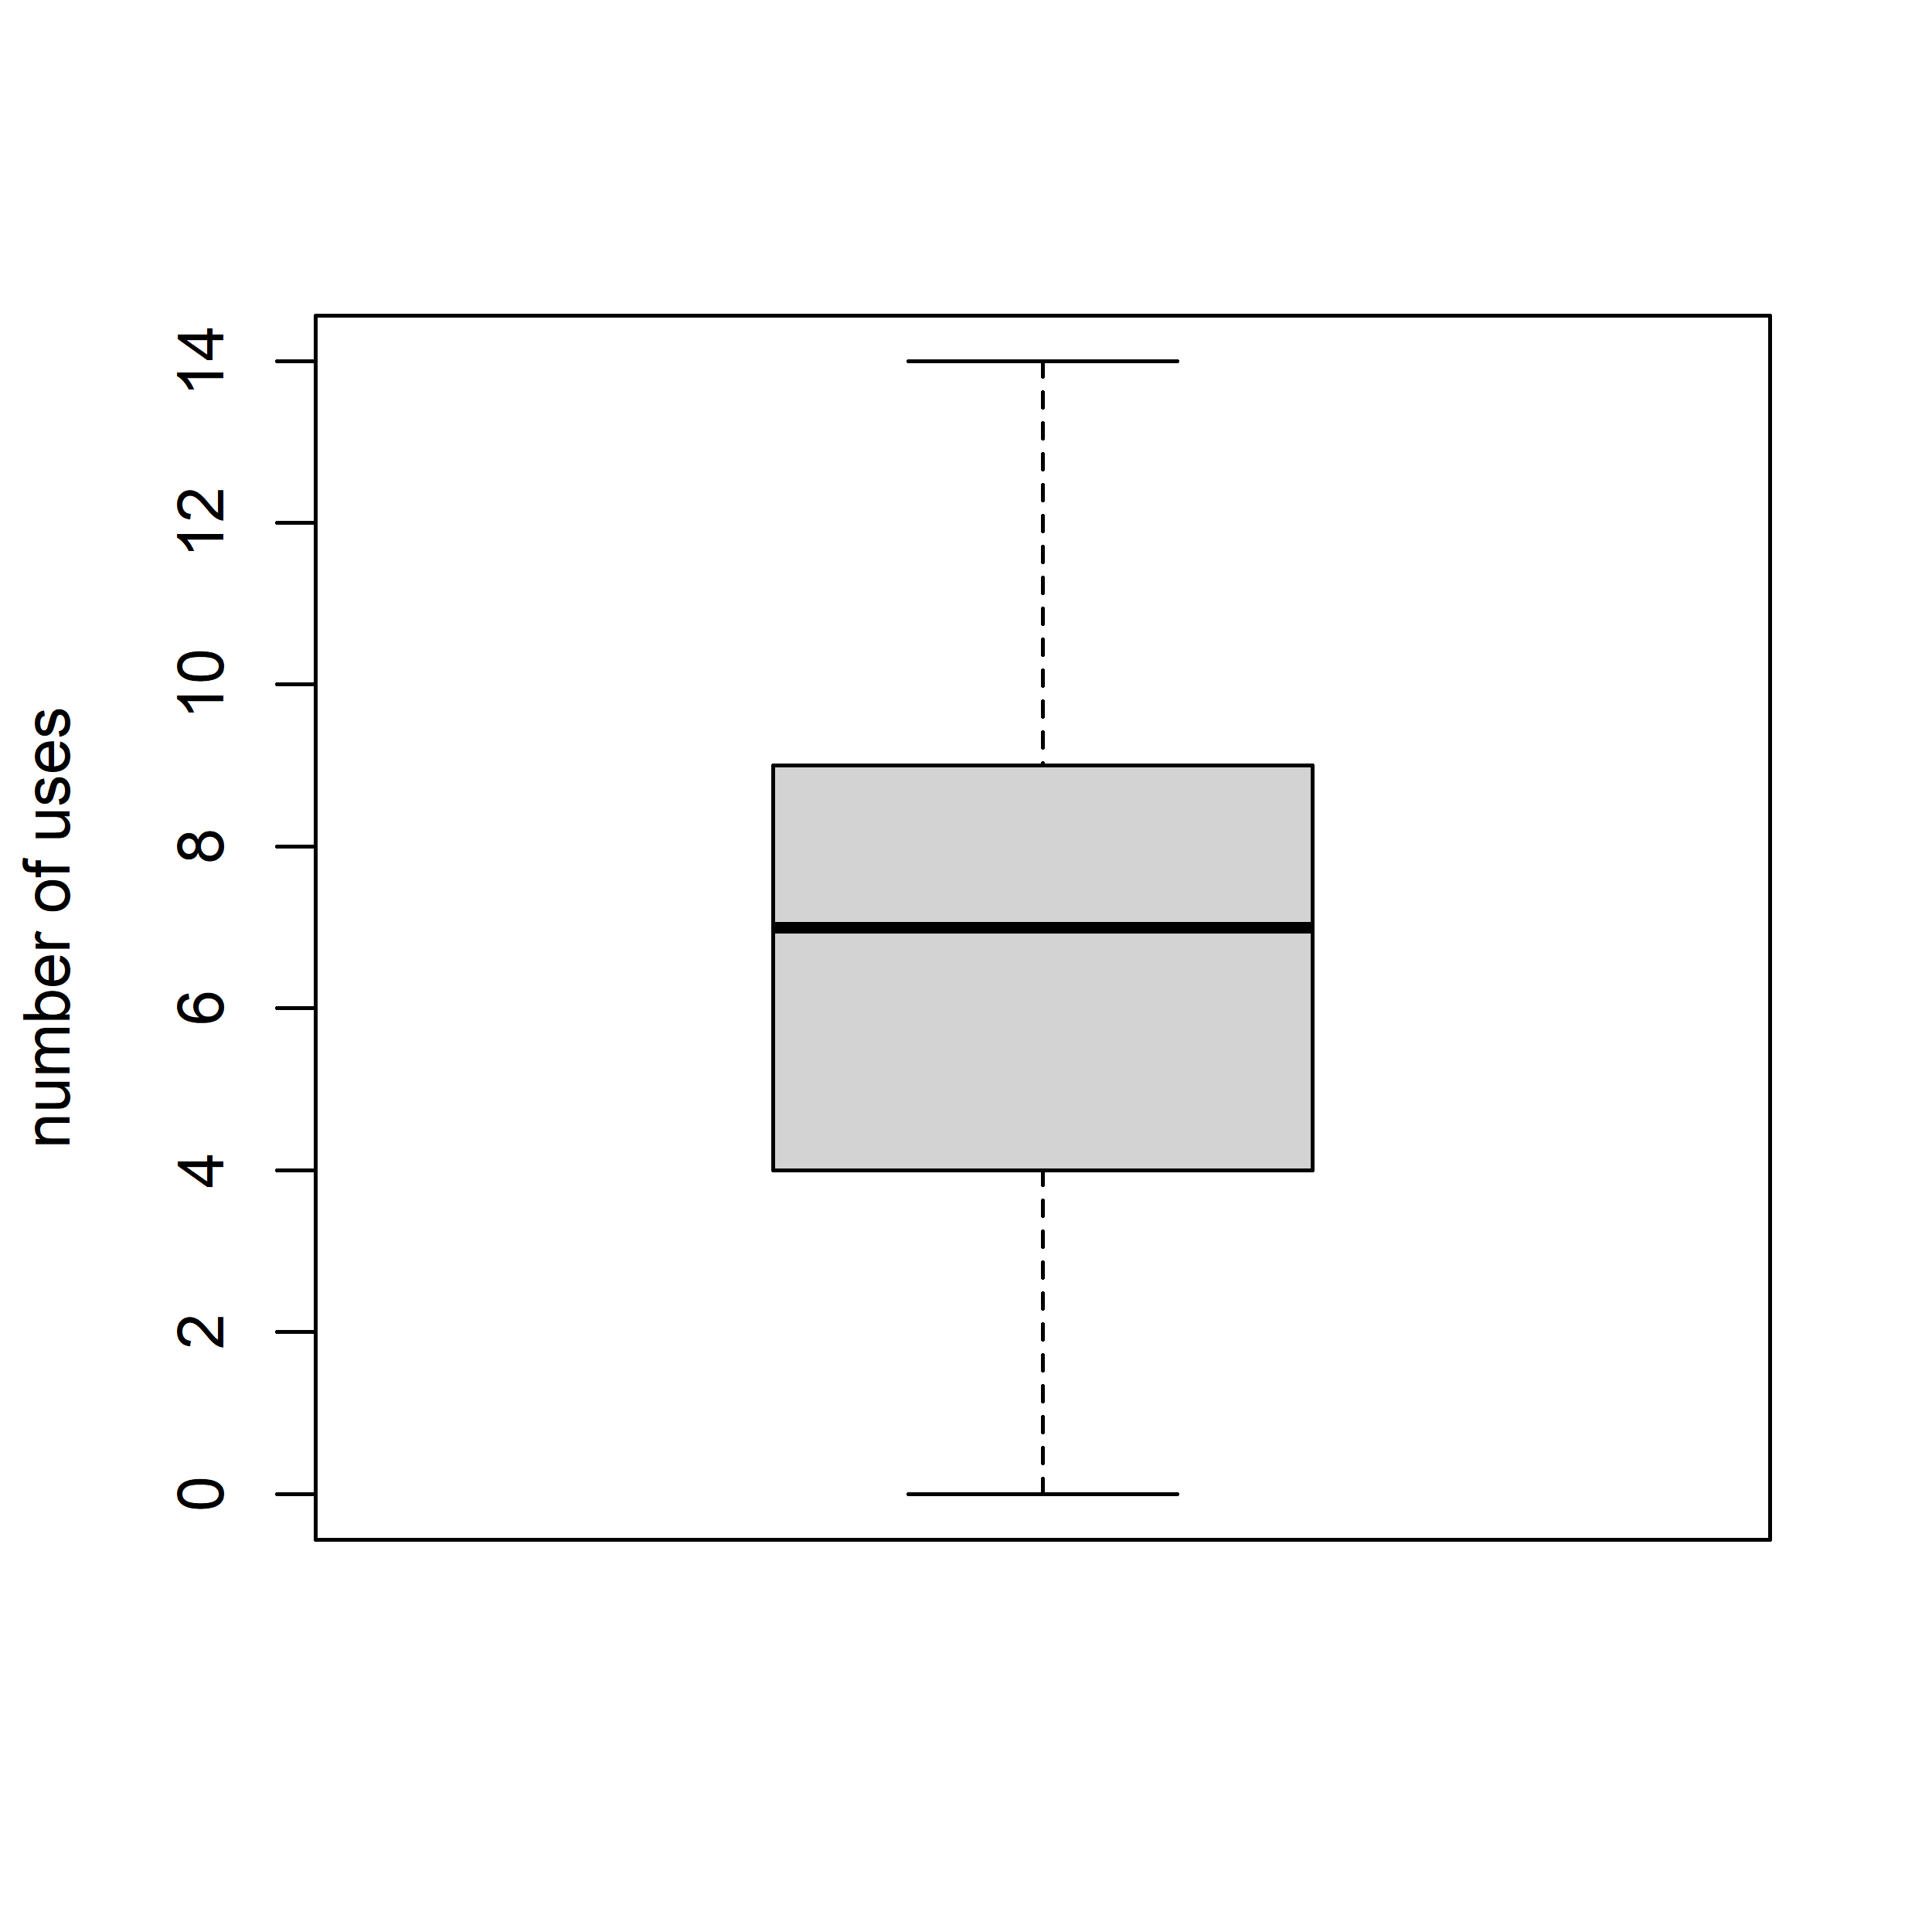
\includegraphics[scale = 0.5]{figures/cal_use_by_person.png}
    \end{figure}
  \end{frame}

  \begin{frame}{Figure: number of correct answers by item}
    \begin{figure}
      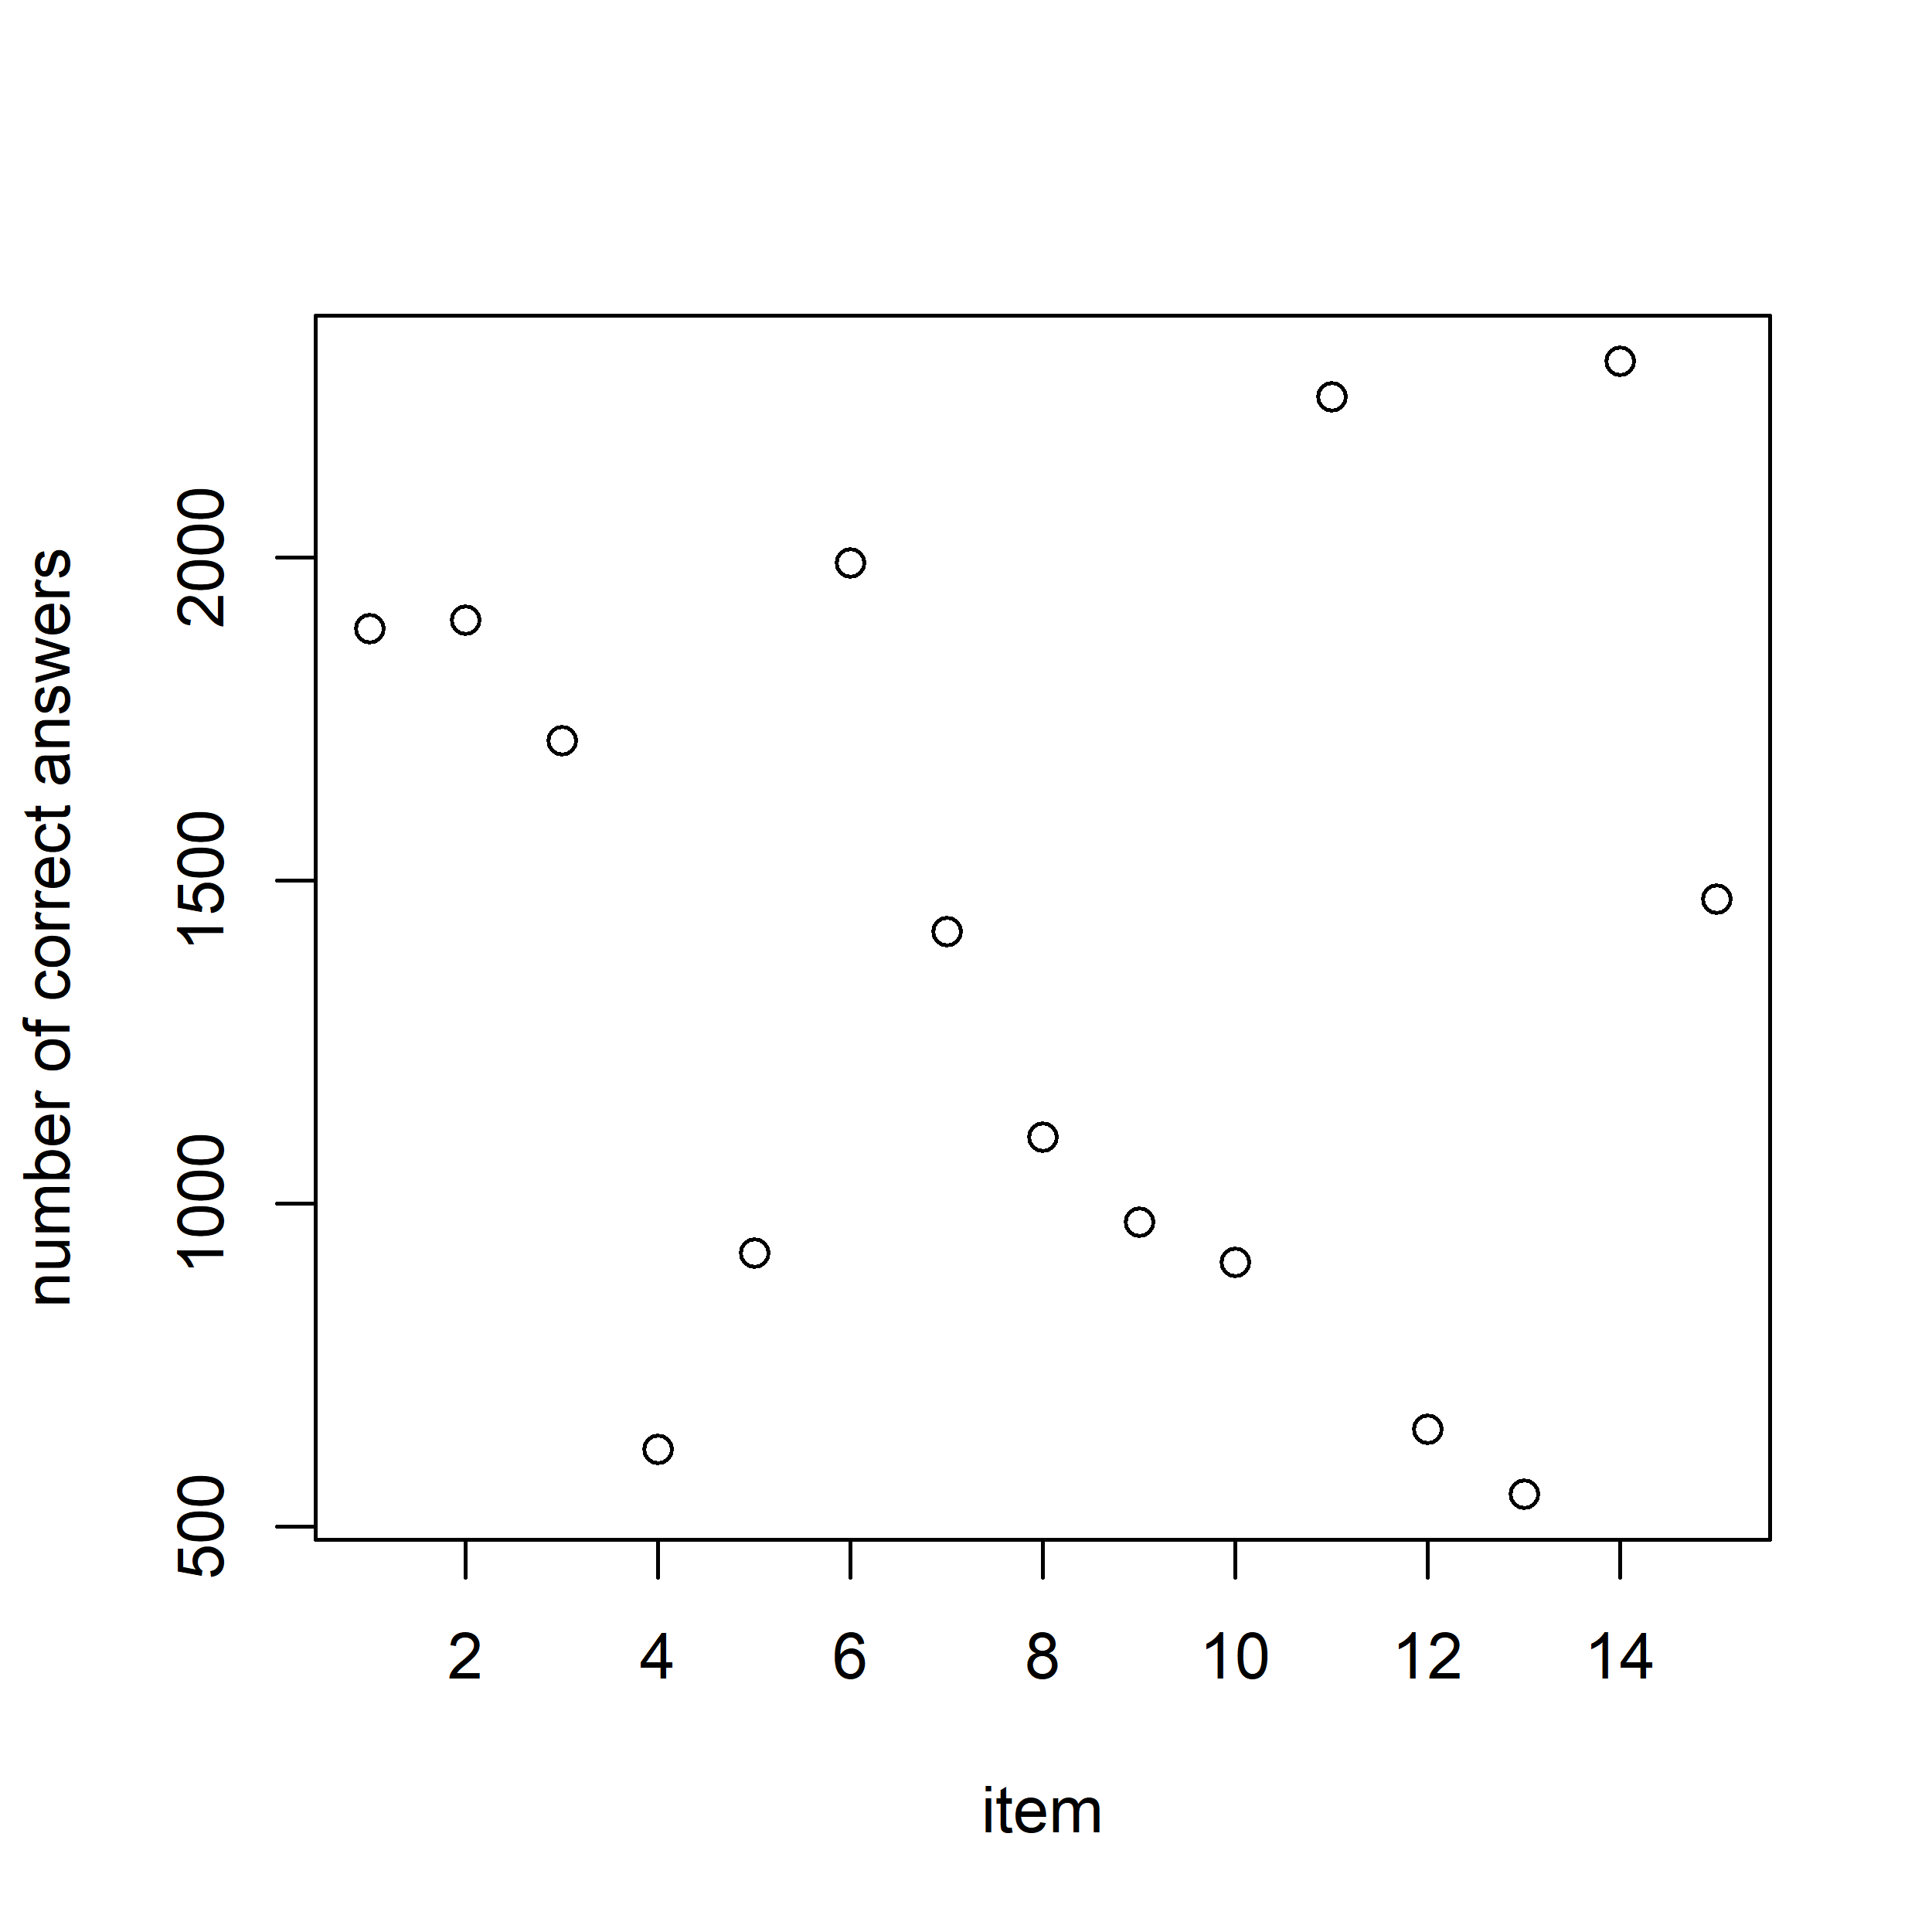
\includegraphics[scale = 0.5]{figures/number_correct_by_item.png}
    \end{figure}
  \end{frame}

  \begin{frame}{Figure: number of correct answers by student}
    \begin{figure}
      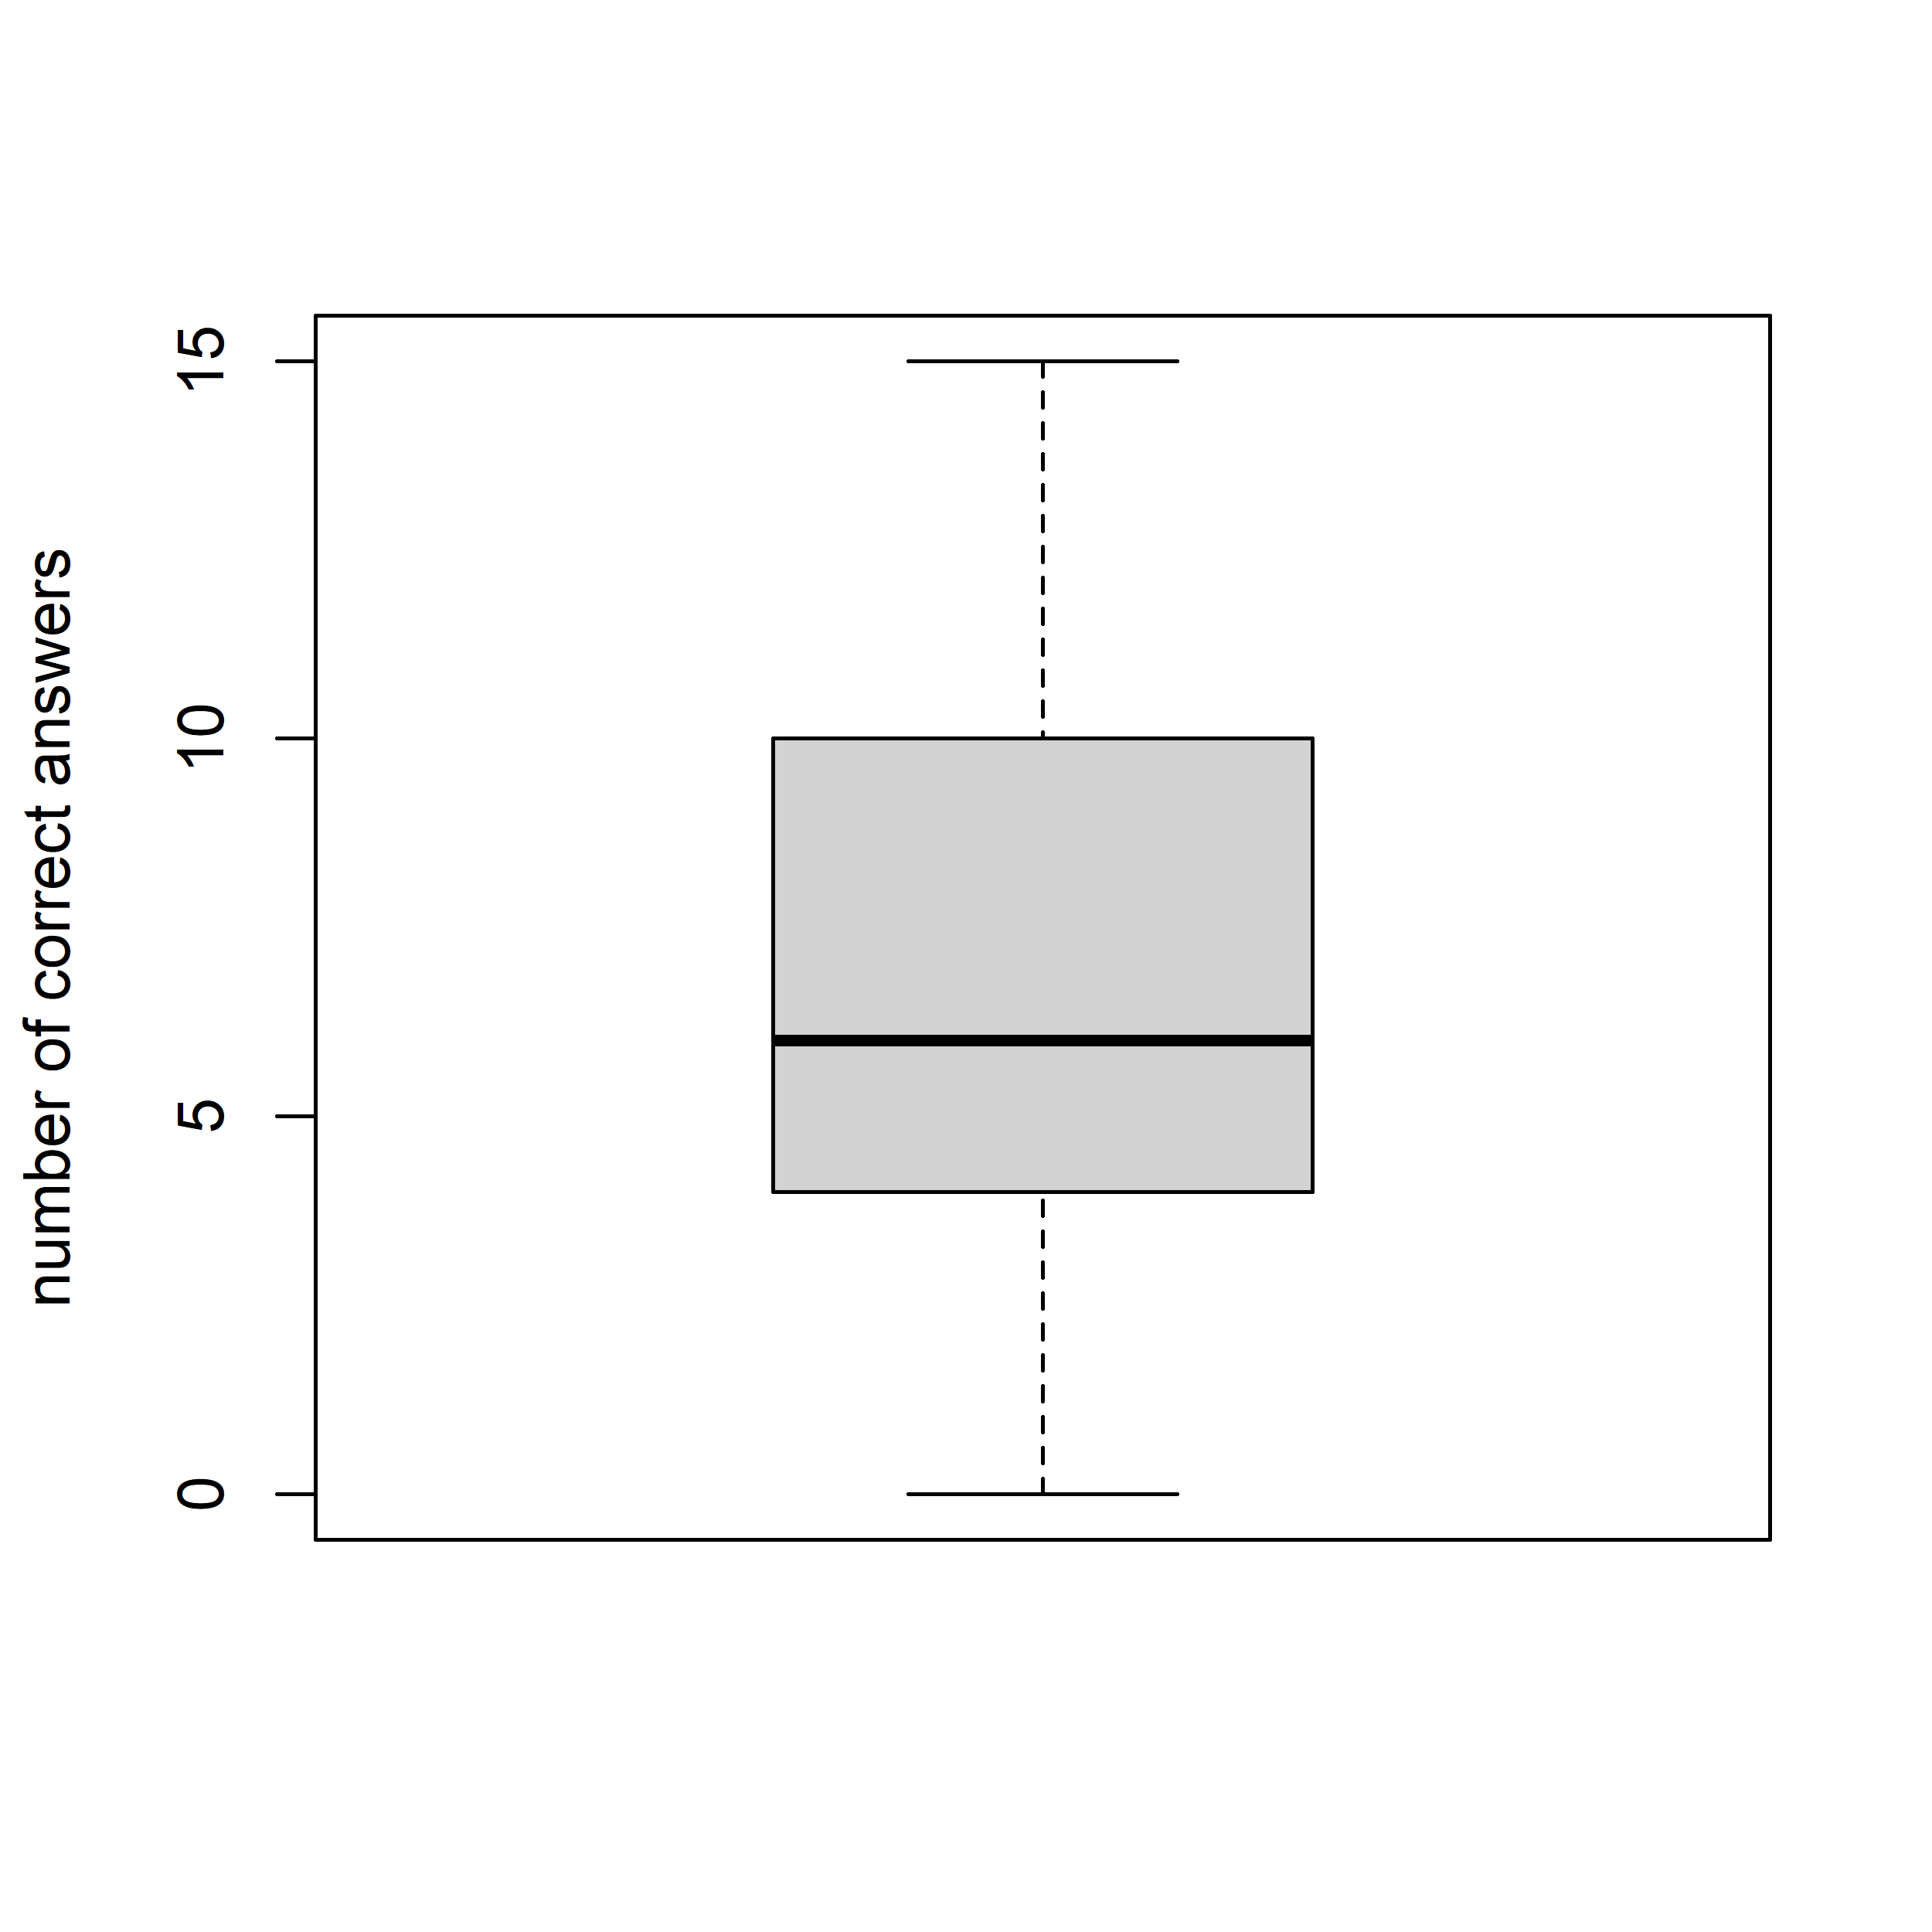
\includegraphics[scale = 0.5]{figures/number_correct_by_person.png}
    \end{figure}
  \end{frame}

  \begin{frame}{Figure: 2D density of raw score and calculator use}
    \begin{figure}
      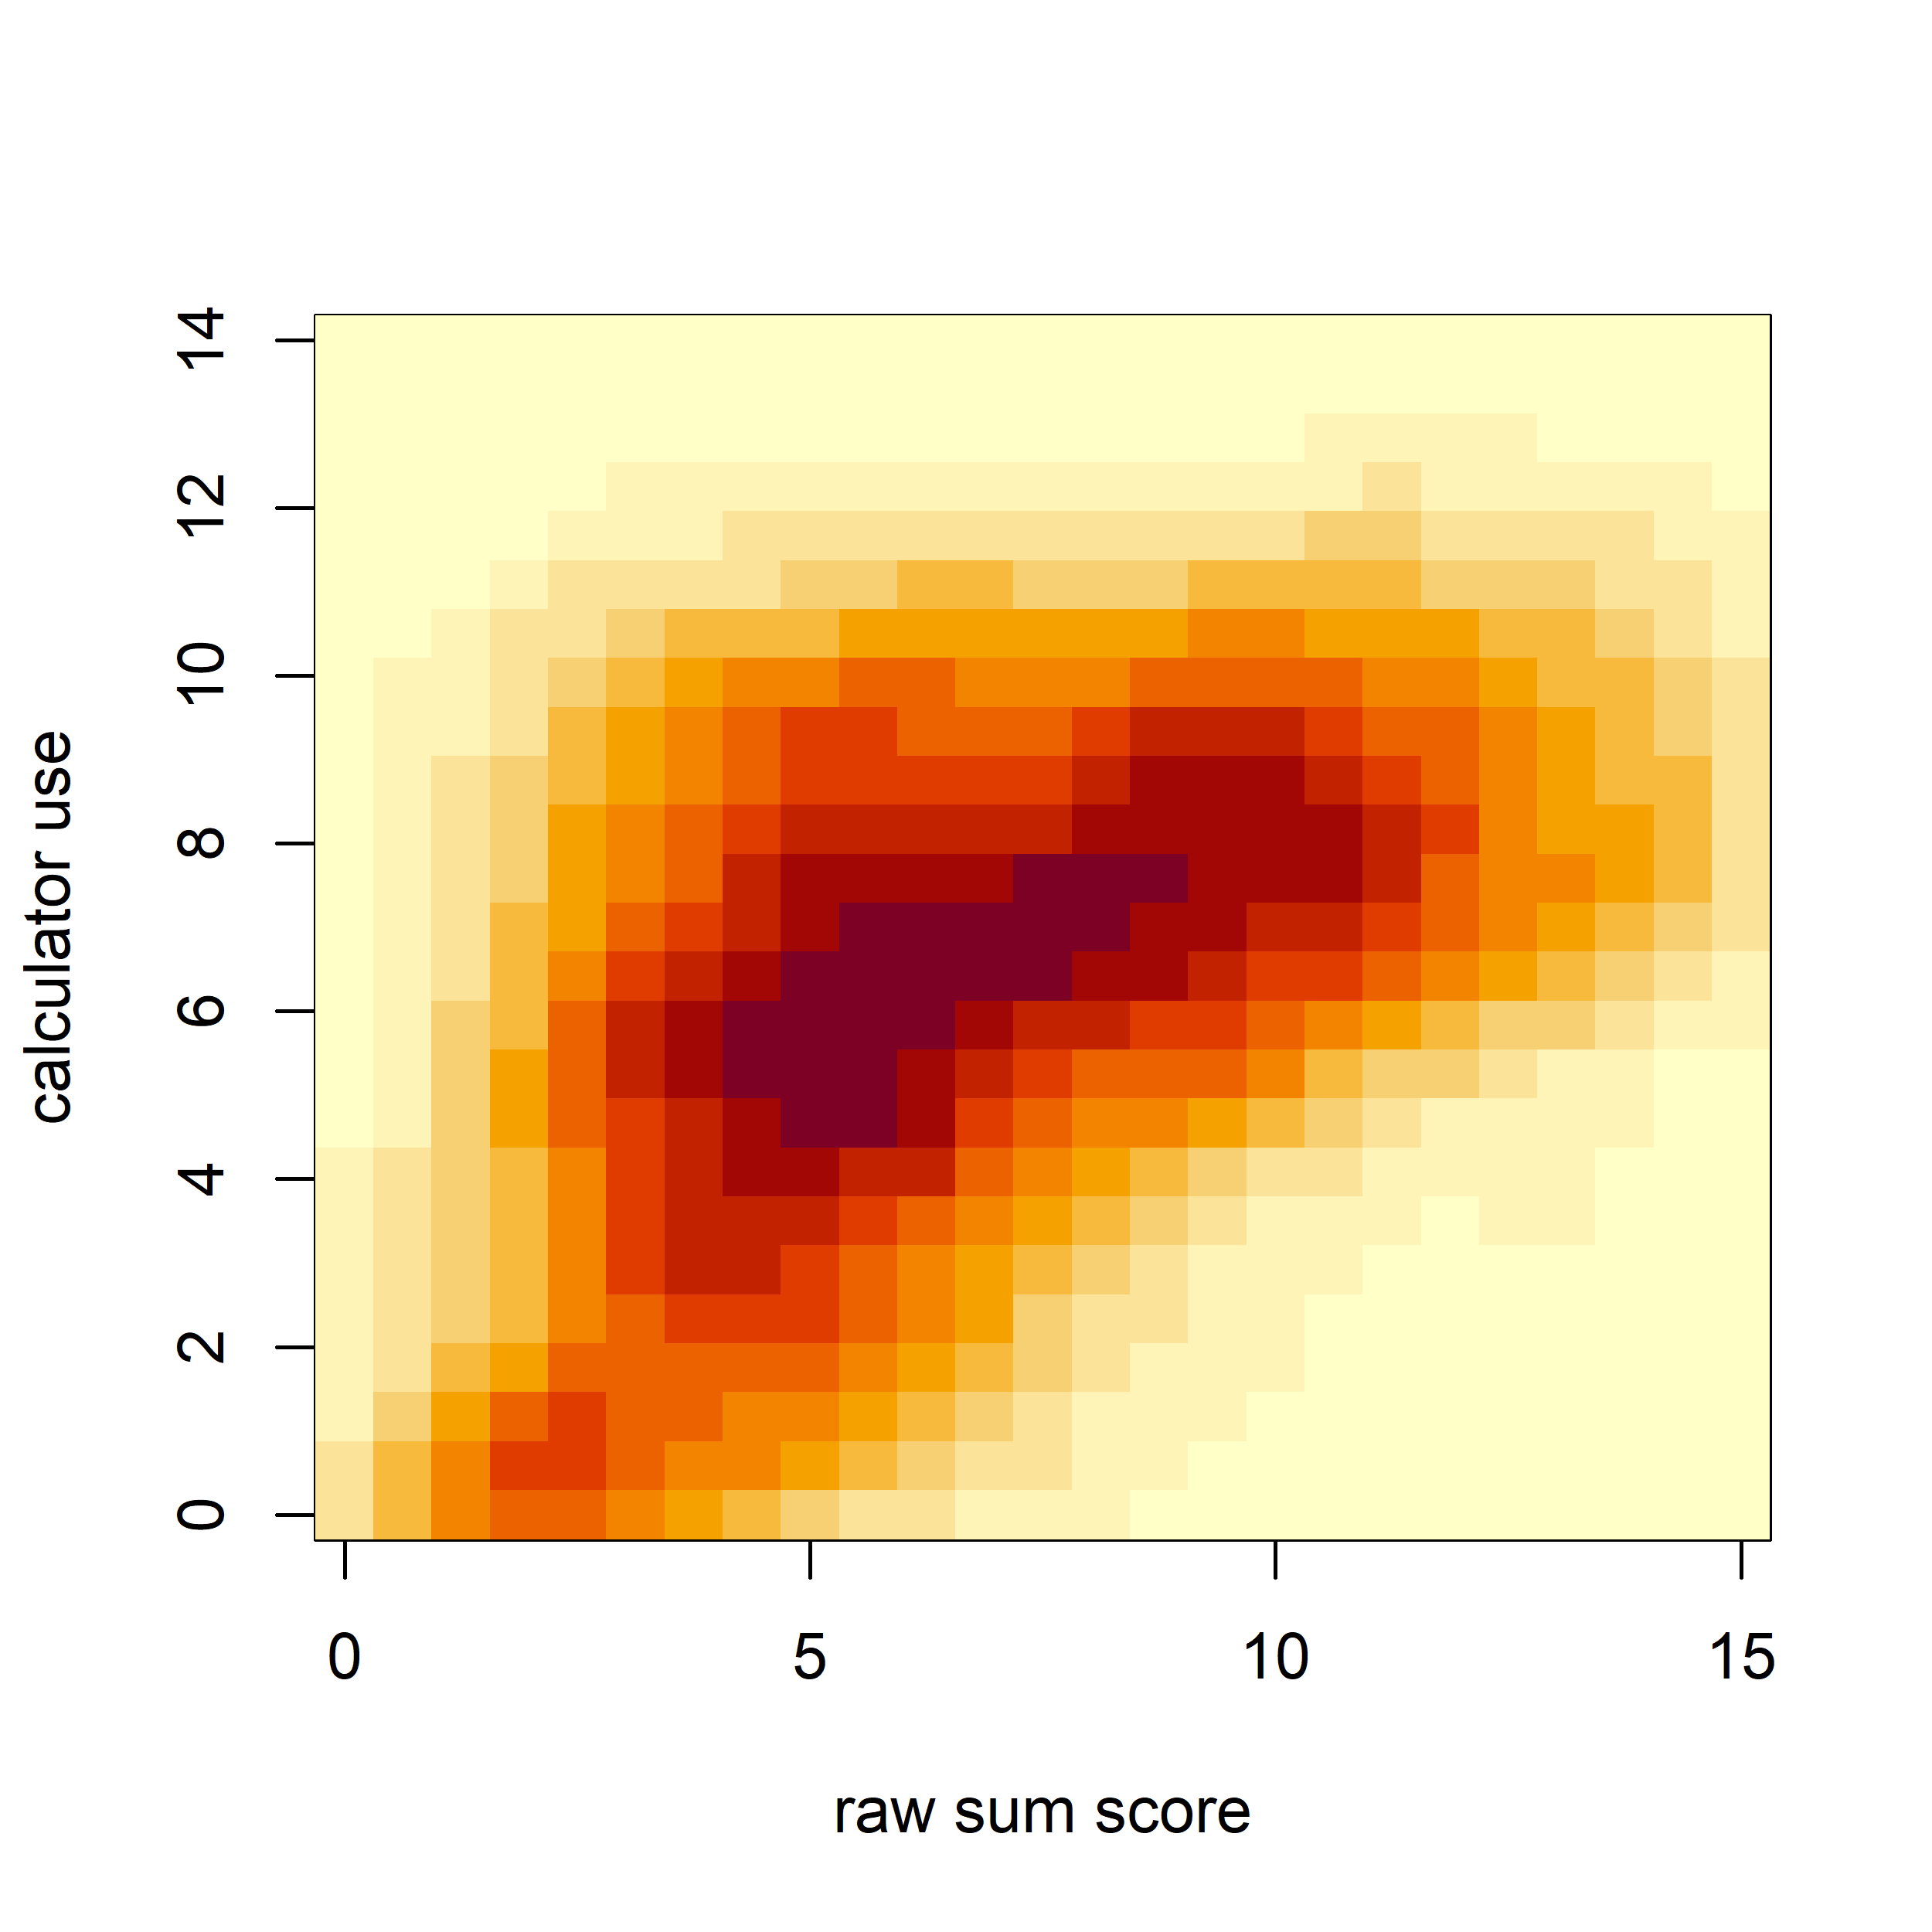
\includegraphics[scale = 0.5]{figures/cor_density.png}
    \end{figure}
  \end{frame}

  \begin{frame}{What do we model?}
    \begin{itemize}
      \item Varying levels of item difficulty 
      \item Varying levels of calculator attractiveness
      \item Varying levels of proficiency
      \item Varying levels of propensity of using the calculator
      \item Correlation between proficiency and calculator propensity
      \item Varying levels of helpfulness of using a calculator (conditional proficiency) 
    \end{itemize}
  \end{frame}

  \section{Model and parameter estimation}
  \begin{frame}{A probabilistic graphical model}
    \begin{figure}
      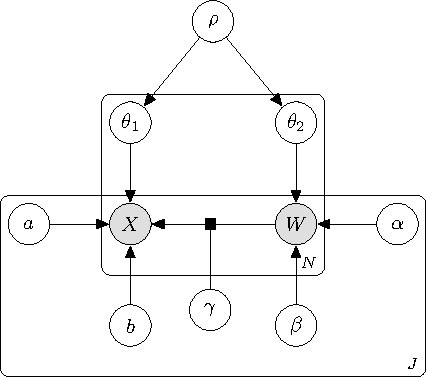
\includegraphics[scale = 0.8]{figures/joint_model_diagram.pdf}
    \end{figure}
  \end{frame}

  \begin{frame}{Conditional independence assumptions}
    The probability of a calculator use is given by
    \begin{equation*}
      P(W_{ij} = 1 | \theta_{i2}, \alpha_j, \beta_j) = \frac{\exp[\alpha_j 
      (\theta_{i2} - \beta_j)]}{1 + \exp[\alpha_j (\theta_{i2} - \beta_j)]}.
    \end{equation*}

    The probability of a correct response is given by
    \begin{equation*}
      P(X_{ij} = 1 | \theta_{i1}, a_j, b_j, w_{ij}, \gamma_j) = \frac{\exp[a_j
      (\theta_{i1} - b_j + w_{ij} \gamma_j)]}{1 + \exp[a_j(\theta_{i1} - b_j + w_
      {ij} \gamma_j)]}.
    \end{equation*}

    \begin{equation*}
      \bm{\theta}_i \sim \Phi\left(\bm{0}, 
      \begin{bmatrix}
      1 & \rho \\
      \rho & 1 \\
      \end{bmatrix}\right).
    \end{equation*}
  \end{frame}

  \begin{frame}{Marginal probability of joint item response and calculator use}
    Marginalizing $\bm{\theta}_i$ over the multivariate normal distribution function $\Phi$, the joint probability of observing $\bm{X}_i = 
    (x_{i1}, x_{i2}, \dots, x_{iJ})$ and $\bm{W}_i = (w_{i1}, w_{i2}, \dots, w_
    {iJ})$ is
    \begin{gather}
    \begin{aligned}
      &P(\bm{X}_i = \bm{x}_i, \bm{W}_i = \bm{w}_i | \bm{a}, \bm{b}, \bm{\alpha}, 
      \bm{\beta}, \bm{\gamma}, \rho)\\ &= \iint \limits_{\bm{\theta}_i \in 
      \mathbb{R}^2} \prod_{j = 1}^{J} P(X_{ij} = x_{ij} | \theta_{i1}, a_j, b_j, w_{ij}, \gamma_j)\\ &P(W_{ij} = w_{ij} | \theta_{i2}, \alpha_j, \beta_j)d\Phi(\bm{\theta}_i;\rho)
    \end{aligned}
    \end{gather}
  \end{frame}

  \begin{frame}{Parameter estimation}
    \begin{itemize}
      \item Observing item response $\bm{x}$ and calculator use $\bm{w}$, we need to estimate $\bm{\alpha}$, $\bm{\beta}$, $\bm{a}$, $\bm{b}$, $\bm{\gamma}$, and $\rho$. 
      \item Direct optimization of the marginal log-likelihood in $5*J + 1$-dimensional space is difficult and requires working with 
      \begin{align*}
        &\sum_{i=1}^{N} \log \iint  \limits_{\bm{\theta}_i \in 
        \mathbb{R}^2} \phi(\bm{\theta}_i;\rho) \prod_{j = 1}^{J} P(X_{ij} = x_{ij} | \theta_{i1}, a_j, b_j, w_{ij}, \gamma_j)\\ &P(W_{ij} = w_{ij} | \theta_{i2}, \alpha_j, \beta_j)d\bm{\theta}_i
      \end{align*}
      \item An Expectation-Maximization (EM) algorithm.
    \end{itemize}
  \end{frame}

  \begin{frame}{Complete data log-likelihood}
    The complete data log-likelihood of the model parameters is
    \begin{equation}
      \log L = \sum_{j=1}^{J}l_j(\alpha_j, \beta_j) + \sum_{j=1}^{J}l_j(a_j,
      b_j,\gamma_j) + \sum_{i=1}^{N} \log \phi(\bm{\theta}_i;\rho),
    \end{equation}
    where
    \begin{equation}
      l_j(\alpha_j, \beta_j) = \sum_{i=1}^{N} w_{ij}\log P_{ij} + (1-w_{ij})\log
      Q_{ij},
    \end{equation}
    and
    \begin{equation}
      l_j(a_j,b_j,\gamma_j) = \sum_{i=1}^{N} x_{ij}\log \dot{P_{ij}} + (1-x_
      {ij})\log \dot{Q_{ij}}.
    \end{equation}
  \end{frame}

  \begin{frame}{Gradients}
    \begin{equation}
    \label{eq:lik_eq_alpha_beta}
      \nabla l_j(\alpha_j, \beta_j) = 
      \begin{pmatrix}
        \frac{\partial l_j}{\partial \alpha_j}\\
        \\
        \frac{\partial l_j}{\partial \beta_j}
      \end{pmatrix}=
      \begin{pmatrix}
        \sum_{i=1}^{N} (w_{ij}-P_{ij})(\theta_{i2}-\beta_j)\\
        \\
        -\sum_{i=1}^{N} (w_{ij}-P_{ij})\alpha_j
      \end{pmatrix},
    \end{equation}
    and
    \begin{equation}
    \label{eq:lik_eq_a_b_gamma}
      \nabla l_j(a_j,b_j,\gamma_j) =
      \begin{pmatrix}
        \frac{\partial l_j}{\partial a_j}\\
        \\
        \frac{\partial l_j}{\partial b_j}\\
        \\
        \frac{\partial l_j}{\partial \gamma_j}
      \end{pmatrix}=
      \begin{pmatrix}
        \sum_{i=1}^{N} (x_{ij} - P_{ij})(\theta_{i1}-b_j+w_{ij}\gamma_j)\\
        \\
        -\sum_{i=1}^{N} (x_{ij} - P_{ij})a_j\\
        \\
        \sum_{i=1}^{N} (x_{ij} - P_{ij})a_j w_{ij}
      \end{pmatrix}.
    \end{equation}
  \end{frame}

  \begin{frame}
    \begin{equation}
    \label{eq:lik_eq_rho}
      \frac{\partial l(\rho)}{\partial \rho} = N\rho^3-\left(\sum_{i=1}^
      {N}\theta_{i1}\theta_{i2}\right)\rho^2 - \left(N - \sum_{i=1}^{N}
      (\theta_{i1}^2+\theta_{i2}^2)\right)\rho - \sum_{i=1}^{N}\theta_{i1}\theta_{i2}
    \end{equation}
  \end{frame}

  \begin{frame}{EM algorithm}
    Start with some initial guess $\bm{\alpha}^{(0)}, \bm{\beta}^{(0)}, \bm{a}^{(0)}, \bm{b}^{(0)}, \bm{\gamma}^{(0)}, \rho^{(0)}$.
    At the $K$th iteration:
    \begin{itemize}
      \item Update posterior distribution for each $\bm{\theta}_i$ given the current parameter estimates.
      \item Update parameter estimates by solving
      \begin{equation}
        E_{\bm{\theta}|\dots}[\nabla l_j(\alpha_j, \beta_j)] = \bm{0},
      \end{equation}
      \begin{equation}
        E_{\bm{\theta}|\dots}[\nabla l_j(a_j, b_j, \gamma_j)] = \bm{0},
      \end{equation}
      and
      \begin{equation}
        E_{\bm{\theta}|\dots}[\frac{\partial l(\rho)}{\partial \rho}] = 0.
      \end{equation}
    \end{itemize}
  \end{frame}

  \begin{frame}
  \begin{itemize}
    \item For derivative based methods to solve the systems of equations (8) and (9), we need to compute the Jacobian matrix of the gradients $\bm{J}_{\nabla l_j(\alpha_j, \beta_j)}$ and $\bm{J}_{\nabla l_j(a_j, b_j, \gamma_j)}$
    \item The third order polynomial in (10) can be solved analytically.
  \end{itemize}
  \end{frame}

  \begin{frame}{Covariance Matrix of the estimator}
    \begin{itemize}
      \item Invert the negative of the Hessian matrix of the marginal log-likelihood, $-\bm{H}^{-1}$. Doable but slow.
      \item Alternatively, we can use the missing information principal,
      \begin{equation}
      -l^{''}(\bm{\zeta}) = E_{\bm{\theta}|\dots}[-l_{c}^{''}(\bm{\zeta})] - E\left[-\frac{\partial^2 \log f(\bm{\theta}|\bm{\zeta})}{\partial \bm{\zeta} \partial \bm{\zeta}^T}\right]
      \end{equation}
    \end{itemize}
  \end{frame}
  
  \section{Results}
  \begin{frame}{Results: item discriminations}
    \begin{table}[!htbp] \centering 
      \caption{} 
      \label{} 
      \scalebox{0.65}{
    \begin{tabular}{@{\extracolsep{5pt}} ccc} 
    \\[-1.8ex]\hline 
    \hline \\[-1.8ex] 
    item & estimate & s.e. \\ 
    \hline \\[-1.8ex] 
    $1$ & $1.254$ & $0.068$ \\ 
    $2$ & $1.233$ & $0.066$ \\ 
    $3$ & $1.992$ & $0.100$ \\ 
    $4$ & $0.583$ & $0.057$ \\ 
    $5$ & $1.654$ & $0.095$ \\ 
    $6$ & $1.420$ & $0.082$ \\ 
    $7$ & $1.120$ & $0.062$ \\ 
    $8$ & $1.027$ & $0.057$ \\ 
    $9$ & $0.990$ & $0.060$ \\ 
    $10$ & $1.560$ & $0.088$ \\ 
    $11$ & $1.375$ & $0.079$ \\ 
    $12$ & $1.752$ & $0.103$ \\ 
    $13$ & $0.923$ & $0.063$ \\ 
    $14$ & $1.504$ & $0.090$ \\ 
    $15$ & $1.869$ & $0.092$ \\ 
    \hline \\[-1.8ex] 
    \end{tabular}}
    \end{table} 
  \end{frame}

  \begin{frame}{Results: item difficulties}
    \begin{table}[!htbp] \centering 
      \caption{} 
      \label{} 
      \scalebox{0.65}{
    \begin{tabular}{@{\extracolsep{5pt}} ccc} 
    \\[-1.8ex]\hline 
    \hline \\[-1.8ex] 
    item & estimate & s.e. \\ 
    \hline \\[-1.8ex] 
    $1$ & $$-$0.563$ & $0.050$ \\ 
    $2$ & $$-$0.639$ & $0.048$ \\ 
    $3$ & $$-$0.267$ & $0.031$ \\ 
    $4$ & $3.421$ & $0.388$ \\ 
    $5$ & $1.455$ & $0.107$ \\ 
    $6$ & $$-$0.528$ & $0.054$ \\ 
    $7$ & $$-$0.551$ & $0.066$ \\ 
    $8$ & $0.558$ & $0.051$ \\ 
    $9$ & $1.025$ & $0.072$ \\ 
    $10$ & $0.783$ & $0.073$ \\ 
    $11$ & $$-$0.970$ & $0.061$ \\ 
    $12$ & $1.473$ & $0.104$ \\ 
    $13$ & $2.168$ & $0.133$ \\ 
    $14$ & $$-$0.486$ & $0.071$ \\ 
    $15$ & $0.035$ & $0.032$ \\ 
    \hline \\[-1.8ex] 
    \end{tabular}}
    \end{table}
  \end{frame}

  \begin{frame}{Results: calculator discriminations}
    \begin{table}[!htbp] \centering 
      \caption{} 
      \label{}
      \scalebox{0.65}{
    \begin{tabular}{@{\extracolsep{5pt}} ccc}
    \\[-1.8ex]\hline 
    \hline \\[-1.8ex] 
    item & estimate & s.e. \\ 
    \hline \\[-1.8ex]
    $1$ & $0.835$ & $0.054$ \\ 
    $2$ & $0.632$ & $0.058$ \\ 
    $3$ & $0.179$ & $0.090$ \\ 
    $4$ & $1.713$ & $0.086$ \\ 
    $5$ & $1.945$ & $0.094$ \\ 
    $6$ & $2.474$ & $0.127$ \\ 
    $7$ & $1.549$ & $0.077$ \\ 
    $8$ & $0.524$ & $0.075$ \\ 
    $9$ & $1.742$ & $0.116$ \\ 
    $10$ & $2.469$ & $0.127$ \\ 
    $11$ & $0.749$ & $0.050$ \\ 
    $12$ & $2.181$ & $0.107$ \\ 
    $13$ & $0.678$ & $0.057$ \\ 
    $14$ & $1.238$ & $0.072$ \\ 
    $15$ & $1.112$ & $0.089$ \\ 
    \hline \\[-1.8ex] 
    \end{tabular}}
    \end{table} 
  \end{frame}

  \begin{frame}{Results: calculator unattractiveness}
    \begin{table}[!htbp] \centering 
      \caption{} 
      \label{} 
      \scalebox{0.65}{
    \begin{tabular}{@{\extracolsep{5pt}} ccc} 
    \\[-1.8ex]\hline 
    \hline \\[-1.8ex] 
    item & estimate & s.e. \\ 
    \hline \\[-1.8ex] 
    $1$ & $0.650$ & $0.060$ \\ 
    $2$ & $2.282$ & $0.193$ \\ 
    $3$ & $15.859$ & $7.907$ \\ 
    $4$ & $$-$0.702$ & $0.039$ \\ 
    $5$ & $$-$0.273$ & $0.031$ \\ 
    $6$ & $$-$0.444$ & $0.030$ \\ 
    $7$ & $$-$0.590$ & $0.039$ \\ 
    $8$ & $4.523$ & $0.605$ \\ 
    $9$ & $1.551$ & $0.066$ \\ 
    $10$ & $$-$0.097$ & $0.028$ \\ 
    $11$ & $$-$0.230$ & $0.057$ \\ 
    $12$ & $$-$0.251$ & $0.030$ \\ 
    $13$ & $1.962$ & $0.154$ \\ 
    $14$ & $$-$1.469$ & $0.072$ \\ 
    $15$ & $2.330$ & $0.144$ \\ 
    \hline \\[-1.8ex] 
    \end{tabular}} 
    \end{table}  
  \end{frame}

  \begin{frame}{Results: calculator effect}
    \begin{table}[!htbp] \centering 
      \caption{} 
      \label{} 
      \scalebox{0.65}{
    \begin{tabular}{@{\extracolsep{5pt}} ccc} 
    \\[-1.8ex]\hline 
    \hline \\[-1.8ex] 
    item & estimate & s.e. \\ 
    \hline \\[-1.8ex] 
    $1$ & $$-$0.017$ & $0.073$ \\ 
    $2$ & $$-$0.259$ & $0.087$ \\ 
    $3$ & $$-$0.191$ & $0.107$ \\ 
    $4$ & $1.200$ & $0.268$ \\ 
    $5$ & $0.973$ & $0.109$ \\ 
    $6$ & $0.229$ & $0.077$ \\ 
    $7$ & $$-$1.017$ & $0.081$ \\ 
    $8$ & $$-$1.113$ & $0.182$ \\ 
    $9$ & $0.785$ & $0.142$ \\ 
    $10$ & $0.027$ & $0.077$ \\ 
    $11$ & $0.186$ & $0.074$ \\ 
    $12$ & $0.468$ & $0.098$ \\ 
    $13$ & $0.981$ & $0.133$ \\ 
    $14$ & $0.830$ & $0.095$ \\ 
    $15$ & $0.159$ & $0.091$ \\ 
    \hline \\[-1.8ex] 
    \end{tabular}}
    \end{table}
  \end{frame}

  \begin{frame}{Results: correlation between proficiency and calculator propensity}
    The correlation $\rho$ is estimated to be $0.6186$ with a standard error of $0.0166$
  \end{frame}

  \section{Model Fit}
  \begin{frame}{Assessment of model fit}
    \begin{itemize}
      \item How do we know our model fits the data?
      \item Absolute fit and relative model fit.
      \item Log-likelihood ratio test against an independent model (no correlation or any calculator effect).
      \begin{equation}
        LRT = -2 \log \left(\frac{L_{ind}(\hat{\omega_{ind}})}{L(\hat{\omega})}\right) = -2 (l_{ind}(\hat{\omega_{ind}}) - l(\hat{\omega}))
      \end{equation}
      \item The log-likelihood for the independent model is $-45425.3$, and the log-likelihood for the joint model is $-44635.4$. But we need to fit $16=15+1$ more parameters.
      \item $LRT = 1579.805$ with $df = 16$. $P-val < 0.0001$.
      \item The joint model very likely fits better.
    \end{itemize}
  \end{frame}

  \begin{frame}{Testing overall model fit}
    \begin{itemize}
      \item The model induces a multinomial distribution, $\bm{\pi}$, for response/process patterns ${\bm{X}, \bm{W}}$.
      \item Intuitively, we can test the residuals between the model induced multinomial probabilities, $\pi$, and the observed probabilities $p$. For example, $\chi^2 = 2N \sum_{c=1}^{C}(\pi_c - p_c)^2/\pi_c$, for $C = K^J$ where $K$ is the number of possible patterns for each item. In this case, $K = 4$.
      \item But the $J-$dimensional contingency table has $K^J = 1,073,741,824$ cells! We don't (will never) have enough data.
      \item We need a method to test the sparse contingency table.
    \end{itemize}
  \end{frame}

  \begin{frame}{Limited information fit statistics}
    \begin{itemize}
      \item Instead of testing $K^J$ cells of $\bm{\pi}$, we can decompose the contingency table into lower order marginal subtables.
      \item $\dot{\bm{\pi}}_r$ is the vector of the $r$th way marginal probabilities with $s_i = \binom{J}{r} (K-1)^r$ cells.
      \item $\bm{\pi}_r = (\dot{\bm{\pi}}_{1}^{'}, \dot{\bm{\pi}}_{2}^{'}, \dots, \dot{\bm{\pi}}_{r}^{'})$, marginal probabilities up to order $r$. We can test residuals $\bm{e}_r = \bm{p}_r - \bm{\pi}_r$.
      \item Marginal residuals have an asymptotic normal distribution, $\sqrt{N}\hat{\bm{e}}_r \overset{d}{\to} N(0, \bm{\Sigma}_r)$.
      \item Consider test statistic $T_r = N\hat{\bm{e}}^{'}_{r} \hat{W} \hat{\bm{e}}_r$, e.g. $\hat{W} = \bm{I}$.
    \end{itemize}
  \end{frame}

  \begin{frame}{P-value}
    \begin{itemize}
      \item $T_r$ asymptotically has a mixture chi-square distribution.
      \item We can use $A\chi_v + B$ to approximate. moment matching and solve for $A, B, v$.
    \end{itemize}
  \end{frame}


\end{document}